In this section, the mobile application used to control the hydrometer will be outlined. The user will interact with the hydrometer application, which will send the request to the server.

\subsection{Control Application}
The mobile control application will be how users interact with the hydrometer after it has been placed inside a brew container. Users will be able to toggle when the hydrometer reads data and be notified of when the resultant specific gravity measurement is of the user's chosen setting.

\begin{figure}[h!]
	\centering
 	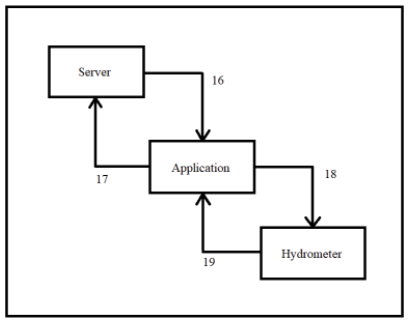
\includegraphics[width=0.60\textwidth]{images/mobile_phone_subsystem}
 \caption{Mobile Phone Subsystem}
\end{figure}

\subsubsection{Assumptions}
Data will be sent via bluetooth, as a constant stream of read-in tilt positions. The phone will have bluetooth capabilities, with an internet connection. The hydrometer itself will not be interacting with the server directly.

\subsubsection{Responsibilities}
The application will be the only way for the web server and hydrometer to communicate. Data will automatically be sent from the application to the server once received. Any return data will be sent in response from the server after processing, or the next time the user loads the application.

\subsubsection{Subsystem Interfaces}
Incoming and outcoming data elements that will pass through the mobile phone subsystem are as follows:

\begin{figure}[h!]
	\centering
 	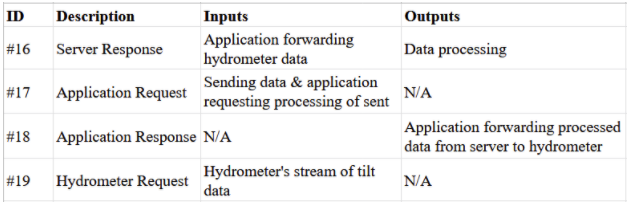
\includegraphics[width=\textwidth]{images/6.1.3_subsystem_table}
 \caption{Mobile Phone Subsystem}
\end{figure}

\subsection{Database subsystem}
The database will be where all data on an hourly/daily basis will be stored. This data will be stored for use and analysis by the user at the time of their choosing.

\subsubsection{Assumptions}
The assumption made for the database is that it will strictly be for analytical purposes. Data stored there will be sorted by hourly and daily. Database syntax will use the SQL syntax.

\subsubsection{Responsibilities}
Database will store all data given to it from the control application. Data stored here is data the user needs to keep track of the brewing process. 

\subsubsection{Subsystem Interfaces}

\begin {table}[H]
\caption {Subsystem interfaces} 
\begin{center}
    \begin{tabular}{ | p{1cm} | p{6cm} | p{3cm} | p{3cm} |}
    \hline
    ID & Description & Inputs & Outputs \\ \hline
    20 & data storage & \pbox{3cm}{data from user} & \pbox{3cm}{N/A}  \\ \hline
    \end{tabular}
\end{center}
\end{table}